\documentclass{article}
\usepackage{amsmath}
\usepackage{tikz}
\usetikzlibrary{positioning}

\begin{document}

\begin{figure}[h]
    \centering
    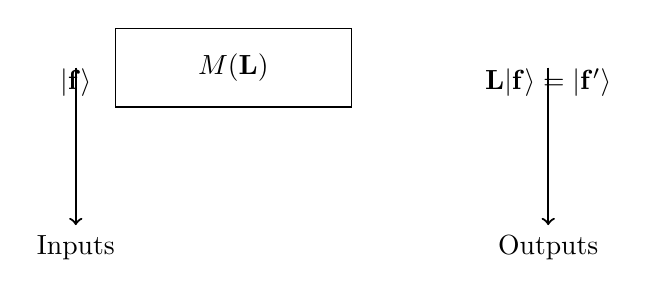
\begin{tikzpicture}[node distance=1cm, auto]
        % Draw lines for the input and output
        \draw[thick] (-2,0) -- node[above] {$|{\bf f}\rangle$} (-2,-1);
        \draw[->, thick] (-2,-1) -- ++(0,-1) node [below] {Inputs};
        \draw[thick] (4,0) -- node[above] {{\bf L}$|{\bf f}\rangle = |{\bf f}'\rangle$} (4,-1);
        \draw[->, thick] (4,-1) -- ++(0,-1) node [below] {Outputs};
        
        % Draw the rectangle for the machine M(L)
        \node [rectangle, draw, minimum width=3cm, minimum height=1cm, align=center] (rect) at (0,0) {$M({\bf L})$};
    \end{tikzpicture}
    \caption{Computational model of a machine $M$ with inputs $|{\bf f}\rangle$ and outputs ${\bf L}|{\bf f}\rangle = |{\bf f}'\rangle$.}
    \label{fig:computational_model}
\end{figure}

\end{document}